\section{Results}

To understand how much more performance we were getting out of our parallel implementations of the shallow water problem we ran strong and weak scaling studies of our code when run on the Xeon E5. For strong scaling studies we ran a number of problem sizes (square problems, this is side length): 360, 720, 1080, 1440, 1800, 2160, 2520, 2880. We chose multiples of 360 as it is the LCM of the square roots of the number of threads we planned on running. For the Xeon E5 2620s we ran each n for $1^2,~2^2,~3^2,~4^2,~5^2$ threads. For the Xeon Phi Accelerator boards we ran each n for $1^2,~2^2,~3^2,~4^2,~5^2,~6^2,~8^2,~9^2,~10^2,~12^2,~15^2$ threads. We plot speedup by having a multi-line plot with a line for each problem size ($N$), the x-axis corresponds to number of threads and the y-axis to speedup.

To generate speedup we compared performance of the E5s versus Professor Bindel's code from the point at which we forked it. We did the same for the Phis as we did for the E5s, but also calculated speedup against a single thread of our code offloaded to the Phis.

Weak scaling was only calculated for a problem size per processor of 360-by-360. We once again used the baselines described in the previous paragraph to calculate speedup for the E5s and the Phis.

\begin{figure}[h!]
\centering
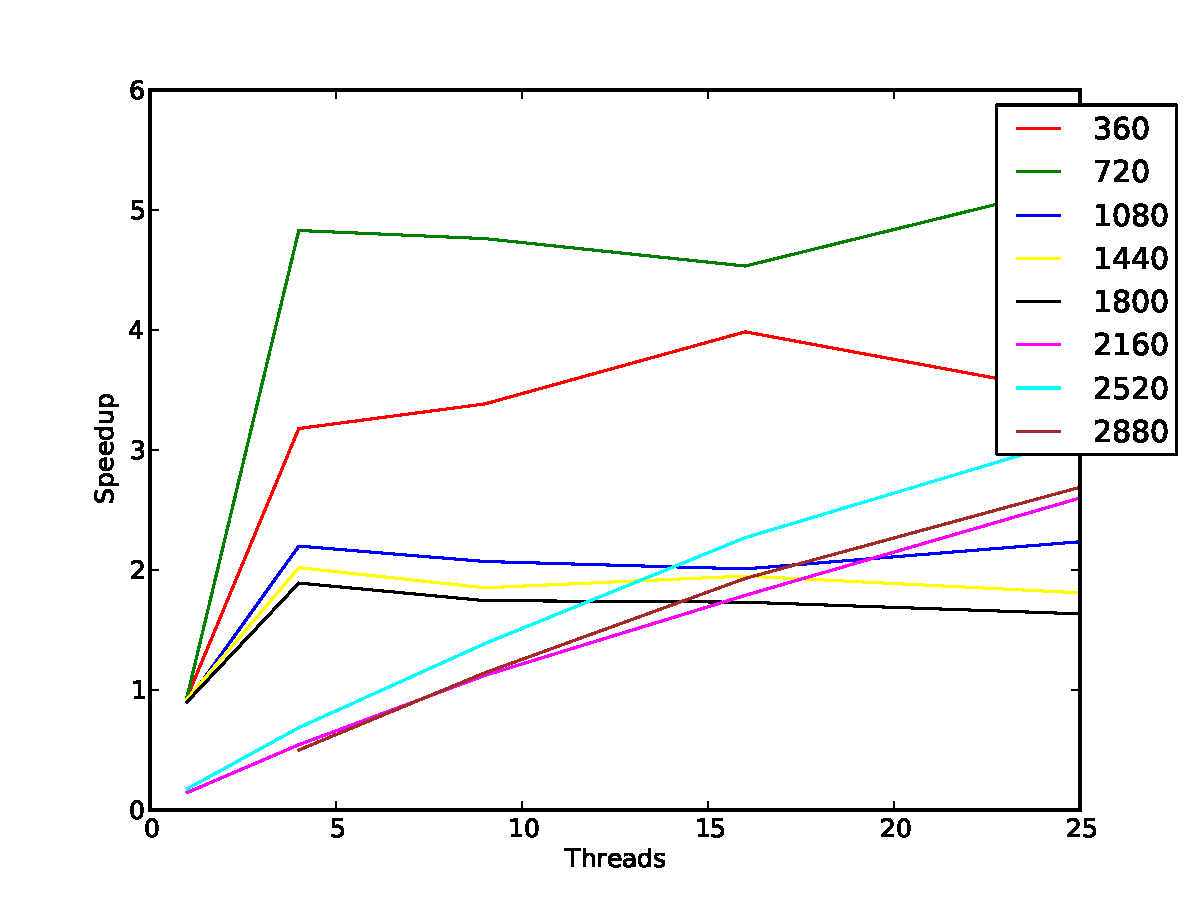
\includegraphics[width=0.5\linewidth]{e5_strong_bindel_baseline.pdf}
\caption{Strong scaling speedup for running on the Xeon E5 2620s. Baseline for calculating speedup is Professor Bindel's code from the point at which we forked it.}
\label{fig:strong-e5}
\end{figure}

\subsection{Xeon E5 Performance}

We began our analysis by studying how our code performed on the Xeon E5 cores. We found that we could get some speedup over Professor Bindel's code, but as the problem size increased speedup actually got smaller (Figure~\ref{fig:strong-e5}). In particular we get relatively large strong scaling speedup for $n=\{360,720\}$, peaking at over 4 for 720, and over 3 for 360. Larger than 720 though and the speedup for any size barely peaks over 2.

This is surprising as typically speedup is better on larger problems where more time can be spent in parallel relative to the amount of time needed for synchronization. We believe this is likely because once the problem size goes beyond 720, each subdomain has poor cache performance as the subproblems are unlikely to fit well in the cache. In particular performance is likely poor with each of the L3 caches which are shared among 12 hardware threads each.

\subsubsection{Weak Scaling}
\begin{figure}[h!]
\centering
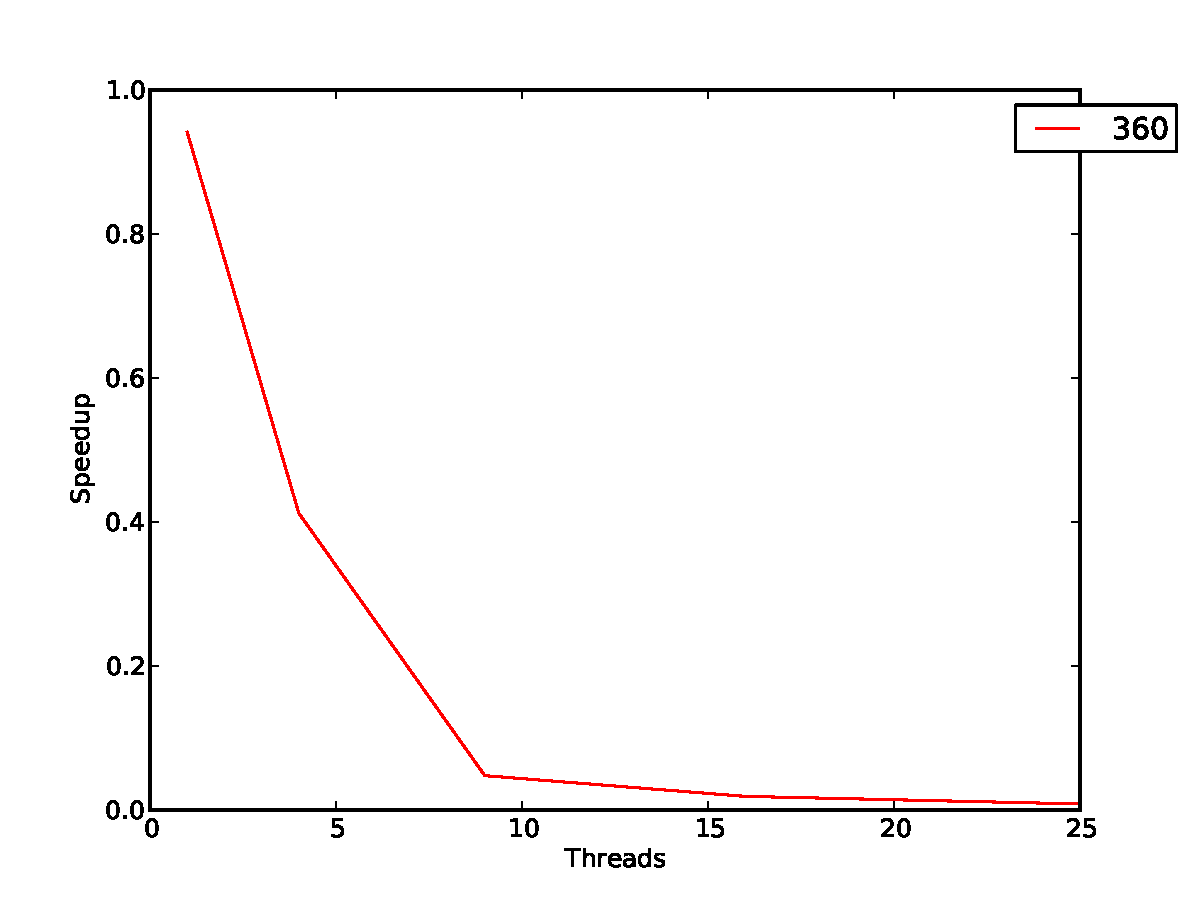
\includegraphics[width=0.5\linewidth]{e5_weak_bindel_baseline.pdf}
\caption{Weak scaling speedup for running on the Xeon E5 2620s. Baseline for calculating speedup is Professor Bindel's code from the point at which we forked it.}
\label{fig:weak-e5}
\end{figure}

When we examine our speedup when doing weak scaling we can see that when each subproblem is fixed at size 360 we quickly lose speedup per core (Figure~\ref{fig:weak-e5}). This is likely due to the dropoff in speedup on problems larger than 720 where cores start competing for L3 cache space and having problems with cache performance.

\subsection{Xeon Phi Performance}

\subsubsection{Strong Scaling}
\begin{figure}[h!]
\centering
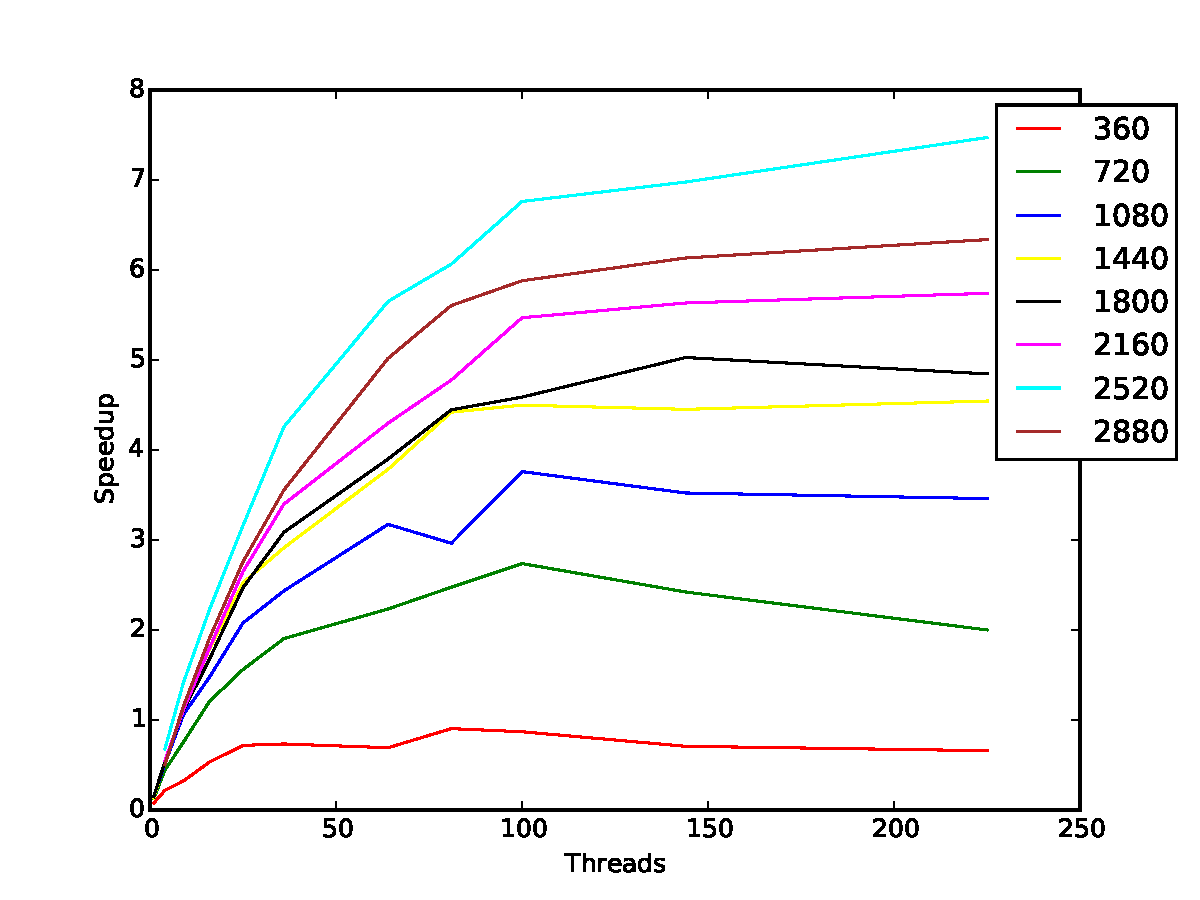
\includegraphics[width=0.5\linewidth]{mic_strong_bindel_baseline.pdf}
\caption{Strong scaling speedup for our offloaded Phi code. Baseline for calculating speedup is Professor Bindel's code from the point at which we forked it.}
\label{fig:strong-mic-bindel}
\end{figure}

To examine the performance of our code when offloaded to the Phis we first examined how the speedup changed for various $n$ and number of threads using strong scaling. The baseline for calculating speedup is Professor Bindel's single threaded code at the point at which we forked it (Figure~\ref{fig:strong-mic-bindel}).

For each $n$ we get a nice logarithmic curve in Figure~\ref{fig:strong-mic-bindel} that shows speedup quickly rising over the first few number of threads sampled and starting to level off as we increase over 100 threads. Further as $n$ increases the speedup generally increases at all number of threads. Speedup peaks at a little under 8 for 225 threads with $n=2520$.

These results are good, though perhaps a little lower than we would like. We likely do not see speedup increases of greater than 10 because Professor Bindel's code is already very fast given that most of it is vectorized, further our vectorization improvements (aligning arrays) had to be discarded in order to get Phi offloading to work. Further, as expected, speedup on the Phis was greater than on the main nodes. This is expected as the simulation is very local and being able to scale to 100s of threads allows us to take huge advantage of the simulations local nature.

\begin{figure}[h!]
\centering
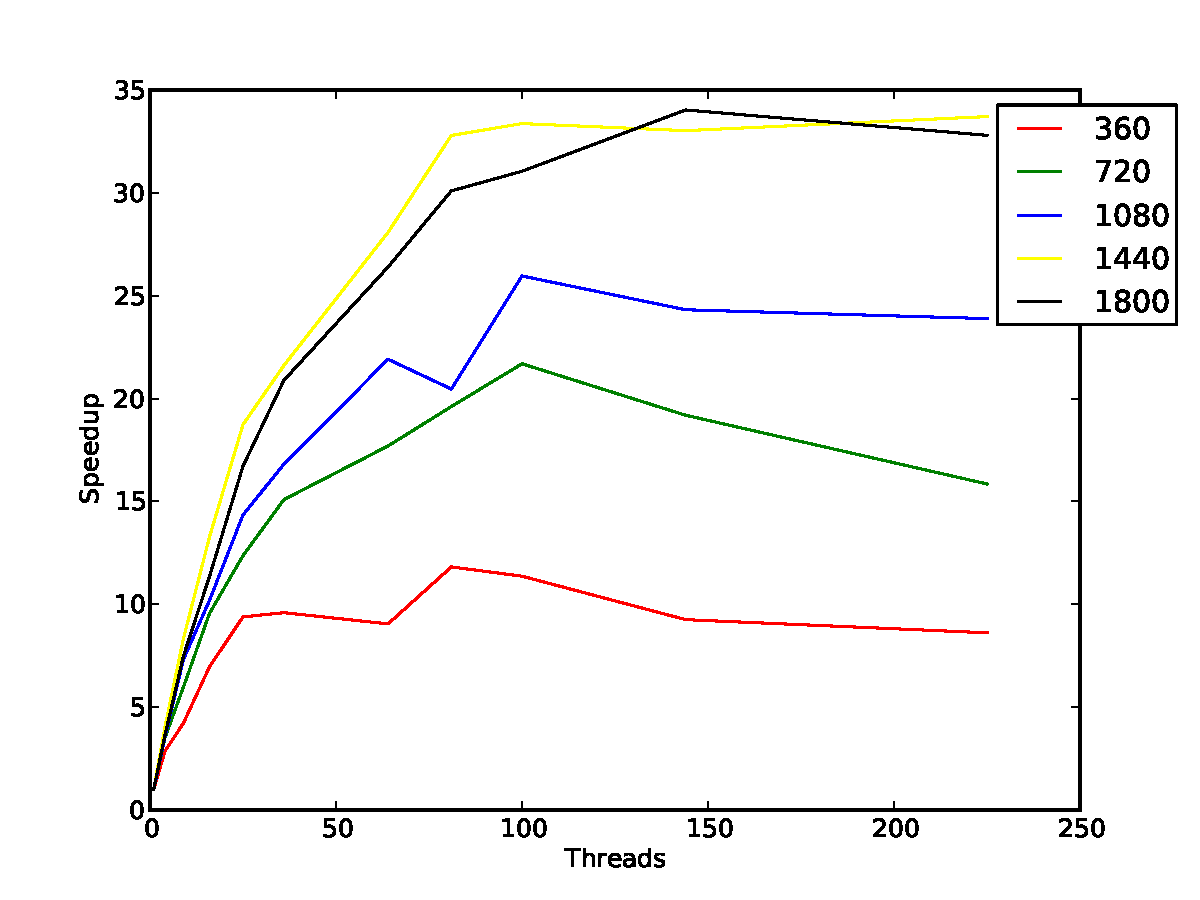
\includegraphics[width=0.5\linewidth]{mic_strong_mic_baseline.pdf}
\caption{Strong scaling speedup for our offloaded Phi code. Baseline for calculating speedup is our code running a single thread offloaded to the Phis.}
\label{fig:strong-mic-mic}
\end{figure}

Too see how much our code obtained a speed-up over itself on the Phis we ran a strong scaling study with the baseline being a single thread of our code offloaded to the Phi boards. The results for this are shown in Figure~\ref{fig:strong-mic-mic}.

We were unable to run this study for as large as $n$ as in the previous study because our single-threaded code on large $n$ would not run fast enough on the Phis (this is expected as a single core of the Phis runs at approximately $1GHz$). In this scaling study we see much larger speedup than we did when compared to Professor Bindel's code. This is expected as a single threaded version of our code can only take advantage of 1 core of the Phi's which results in slow executions.

\subsubsection{Weak Scaling}
\begin{figure}[h!]
\centering
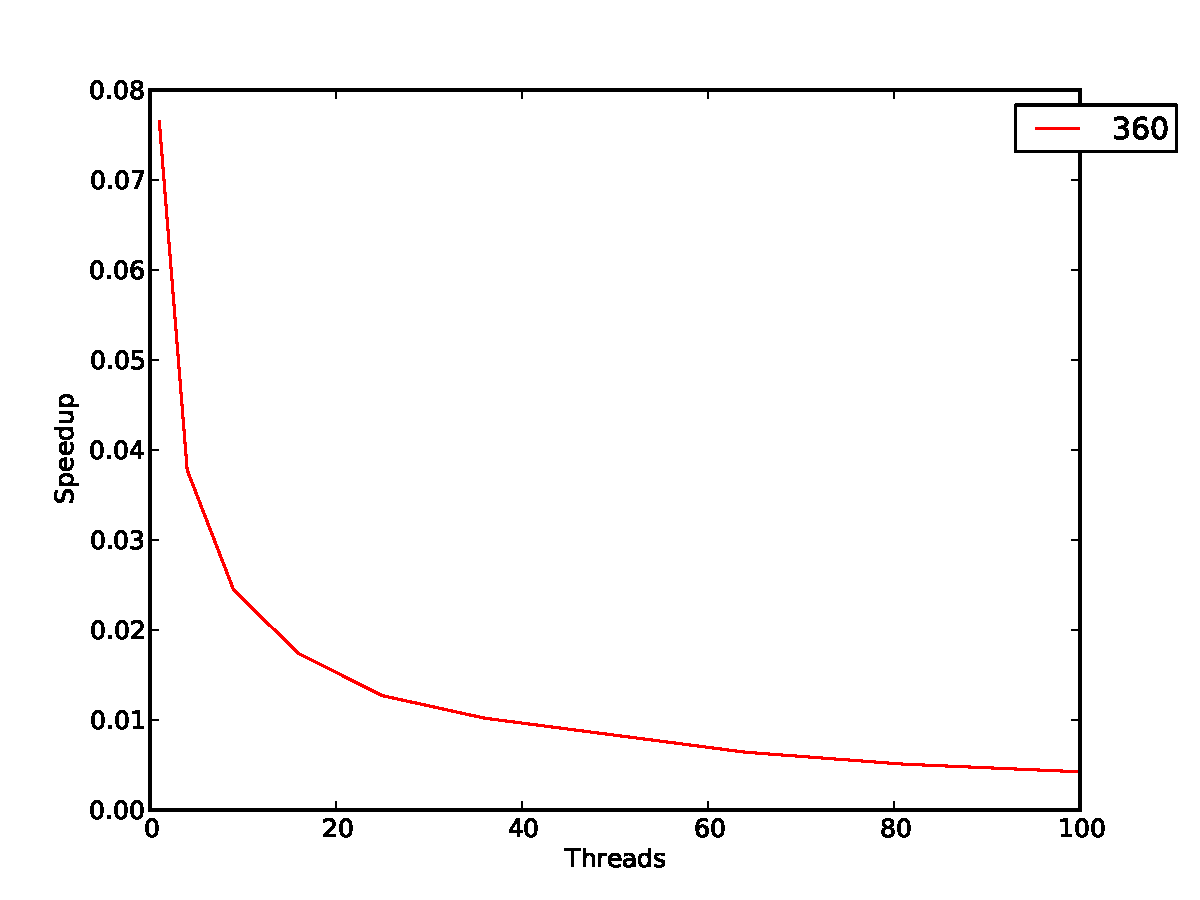
\includegraphics[width=0.5\linewidth]{mic_weak_bindel_baseline.pdf}
\caption{Weak scaling speedup for our offloaded Phi code. Baseline for calculating speedup is Professor Bindel's code from the point at which we forked it.}
\label{fig:weak-mic}
\end{figure}

We also did a weak scaling study of our Phi code (Figure~\ref{fig:weak-mic}), with a baseline of Professor Bindel's code. We find that speedup when problem size is fixed to 360 per thread is very low. This is unsurprising as a single core of the Phis runs at approximately $1GHz$ as compared to a peak speed of $3.2GHz$ per core of the E5 2620s.

\subsection{Batch size Performance}

\begin{figure}[h!]
\centering
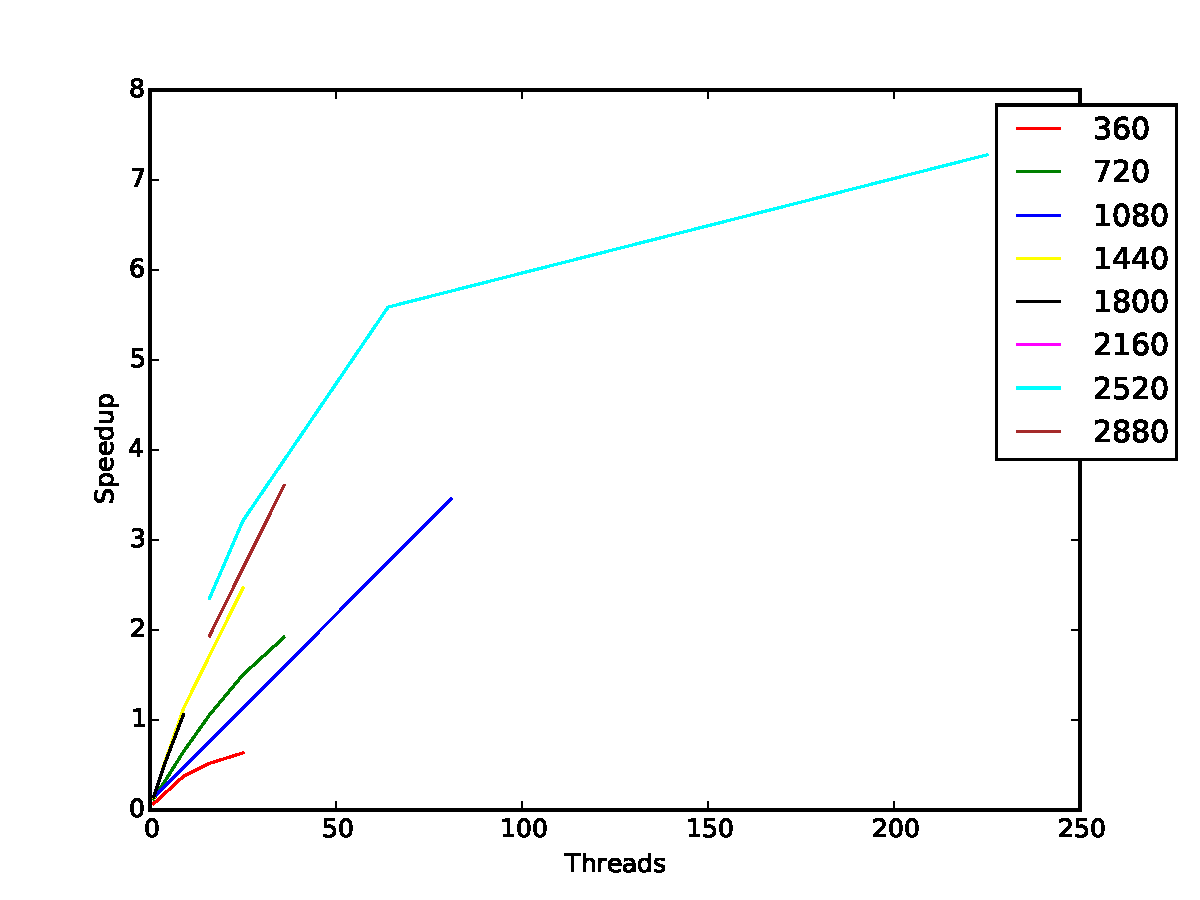
\includegraphics[width=0.5\linewidth]{mic_strong_bindel_baseline_batchsize2.pdf}
\caption{Strong scaling speedup for our offloaded Phi code with a batch size of 2. Baseline for calculating speedup is Professor Bindel's code at the point where we forked it. We can see that speedup is slightly worse than our speedup for batch size of 1.}
\label{fig:batch2}
\end{figure}

We were also interested in how our code performed when we increased batch size on the Xeon Phi boards. We found that when we increased batch size to two rather than 1 (so 4 steps rather than 2 steps), that our total time was actually slightly worse, because most results were worse, we show only one size (1440) in Figure~\ref{fig:batch2} for reference. This is likely because there are few barriers in our code (one after our speed calculation, one after our copy and compute steps calculation, one after our synchronize section) and no single-threaded sections which take large computation time. Thus synchronization wasn't all the expensive and the extra work (in terms of more ghost cells that have to be calculated for) does not outweigh the decreased synchronization frequency.

Furthermore it is likely that because we have to back-off our dt when doing a batch size of moer than 1 in order to be conservative and not violate the CFL constraint we must do more steps total for our simulatino to complete which means more simulation work is done. Further a larger batch size potentially leads to many extra steps taken near the end of a simulation when a smaller number of steps would suffice.
